\section{Processamento de Linguagem Natural}
\label{sec:chap03_pln}
O \glsfirst{pln} é um campo da Ciência da Computação, \glsfirst{ia} e Linguística que explora a forma como os computadores podem ser usados na compreensão, manipulação e geração automática da linguagem natural, em forma de texto ou voz~\parencite{nlp, applied_natural_language_processing_with_python, pln_extracao_conhecimento}. Nos últimos anos, a área tem-se tornado bastante popular com o acesso fácil a informação através da Internet, estando presente em implementações de \textit{chatbots}, verificadores ortográficos em telemóveis e assistentes de \gls{ia} nos \textit{smartphones}, tais como a Cortana\footnote{Disponível em \url{https://www.microsoft.com/en-us/cortana}.} ou Siri\footnote{Disponível em \url{https://www.apple.com/siri/}.}~\parencite{pln_extracao_conhecimento, applied_natural_language_processing_with_python}. 

\subsection{História}
O início do \gls{pln} remonta aos anos 40, com o desenvolvimento da Ciência da Computação, aliada aos avanços na Linguística, que levou ao aparecimento da teoria da linguagens formais. Muito sucintamente, esta teoria consiste na modelação de estruturas complexas e respetivas regras, ou seja, permitem especificar e reconhecer linguagens a partir de modelos matemáticos (\exempligratia{um alfabeto é uma estrutura simples, a qual é constituída por letras que podem formar palavras, em diferentes idiomas}). Por outro lado, os avanços na \gls{ia}, particularmente com o modelo \gls{slp} apresentado na Figura~\ref{fig:slp}, também contribuíram para este campo~\parencite{applied_natural_language_processing_with_python}. O \gls{slp} é a base dos modelos neuronais usados nos dias de hoje. Warren McCulloch e Walter Pitts propuseram este modelo, baseado na analogia entre células nervosas (neurónios) e os processos computacionais, que permite computar a soma dos pesos ($w_{ni}$) associados a cada entrada ($x_{n}$), dando uma resposta binária consoante o valor da soma ($\sum$) varia de acordo com um determinado valor limite, decidindo se uma determinada ação será executada~\parencite{introduction_theory_neural_computation}.

\begin{figure}[!t]
    \centering
    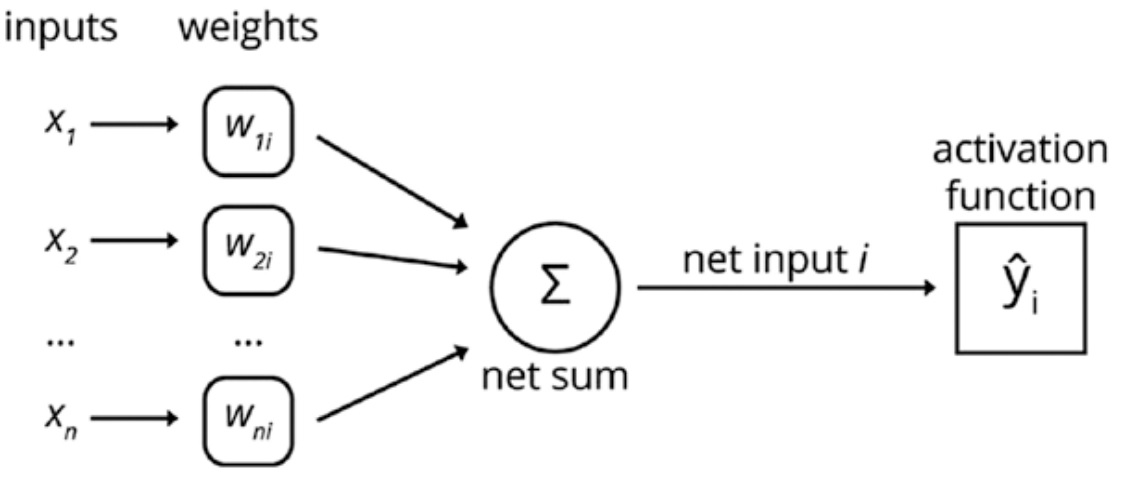
\includegraphics[width=.8\textwidth]{ch03/assets/slp_model.jpg}
    \caption{\glsfirst{slp}, extraído de~\textcite{applied_natural_language_processing_with_python}}
    \label{fig:slp}
\end{figure}

Ao longo dos anos, várias técnicas foram surgindo na tentativa de resolver problemas associados à compreensão da linguagem natural. Mas, nos últimos 20 anos, notou-se o aumento de interesse no \gls{pln}, juntamente com \gls{ml}, sobretudo devido ao aumento do poder computacional e à facilidade de acesso a dados etiquetados através da Internet~\parencite{applied_natural_language_processing_with_python}.

\subsection{Fundamentos}
O cerne de qualquer tarefa de \gls{pln} está relacionado com a compreensão da própria linguagem. O desenvolvimento deste tipo de aplicações incorre em alguns problemas tais como a processo de pensamento, a representação e significado linguístico e/ou conhecimento do domínio, que estão associados à ambiguidade da linguagem natural~\parencite{nlp, pln_extracao_conhecimento}. Por outras palavras, a ambiguidade surge quando não é possível atribuir um significado único a uma dada expressão. Se uma pessoa é capaz de o fazer, baseada na sua experiência, capacidade de interpretação de contexto ou na sua cultura, já um computador não tem essa mesma capacidade~\parencite{pln_extracao_conhecimento}. Por isso, \textcite{nlp} enuncia que, para ser capaz de compreender a linguagem natural, é importante considerar os vários níveis de conhecimento interdependentes que o ser humano usa na extração de significado:

\begin{itemize}
    \item 
    {
        \textit{Nível fonético ou fonológico} -- encarrega-se a pronúncia;
    }
    \item
    {
        \textit{Nível morfológico} -- lida com os \textit{tokens}, ou seja, partes nucleares de um frase (\exempligratia{palavras, sufixos, prefixos, sinais de pontuação, dígitos, entre outros});
    }
    \item
    {
        \textit{Nível léxico} -- trata do significado léxico dos símbolos e análise de partes do discurso;
    }
    \item 
    {
        \textit{Nível sintático} -- lida com a gramática e a estrutura frásica;
    }
    \item
    {
        \textit{Nível semântico} -- encarrega-se de clarificar o significado da frase ou das palavras;
    }
    \item
    {
        \textit{Nível pragmático} -- ocupa-se da relação entre a linguagem e o contexto, ou seja, contempla a relação com o mundo exterior;
    }
    \item
    {
        \textit{Nível de discurso} -- suporta o agrupamento de diferentes frases, identificando a relação entre elas, de forma a compreender o contexto.
    }
\end{itemize}

Um sistema \gls{pln} pode envolver todos ou alguns destes níveis, cujas atividades permitem solucionar pequenas partes de um problema mais complexo. Algumas destas tarefas ou ferramentas incluem técnicas de segmentação de palavras e construção frásica, \textit{parsing} sintático e estatístico, métodos de desenho de modelos de conhecimento estruturados, redes neuronais e modelos de linguagem neuronal~\parencite{nlp, speech_language_processing}.

\subsection{Linguagem Natural para Bases de Dados}
Uma interface de linguagem natural é um componente que aceita expressões de consulta ou comandos em linguagem natural e providencia as respostas apropriadas, ou seja, esta deve ser capaz de traduzir as frases nas respetivas ações para o sistema~\parencite{nlp}. Neste contexto particular, importa explorar as \gls{ilnbd}, as quais permitem os utilizadores executarem pesquisas em bases de dados usando a linguagem natural~\parencite{overview_nlidb_approaches_implementation_airline, novel_approach_building_generic_portable_contextual_nlidb_system}.

As \gls{ilnbd} apresentam um problema clássico na área de \gls{pln} e constitui um campo de estudo em desenvolvimento. Genericamente, a solução inerente a este problema podem ser divida em duas fases: processamento linguístico, em que a frase de pesquisa é mapeada e traduzida para a \textit{query} de \gls{sql} correspondente, usando funções de mapeamento adequadas; processamento na base de dados, na qual é executado a gestão de acesso ao sistema e execução da respetiva consulta~\parencite{overview_nlidb_approaches_implementation_airline}. Este tipo de sistemas é capaz de responder a uma grande variedade de \textit{queries} de linguagem natural mas são pouco usados comercialmente, principalmente pela pouca robustez nas capacidades de processamento de contexto~\parencite{novel_approach_towards_incorporating_context_processing_nlidb}, pela falta de cobertura linguística ou pelo facto de utilizador poder assumir inteligência por parte do sistema~\parencite{survey_nlidb, overview_nlidb_approaches_implementation_airline}. Ainda assim, existem várias vantagens que contribuem para o desenvolvimento deste tipo de aplicações, nomeadamente a facilidade e simplicidade de utilização, o facto de ser mais adequado para questões que envolvem negação ou quantificação ou a sua tolerância a erros gramaticais~\parencite{survey_nlidb, nlidb_brief_review, overview_nlidb_approaches_implementation_airline}.

\begin{figure}[!h]
    \centering
    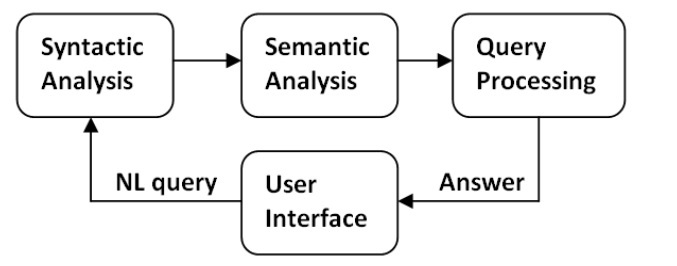
\includegraphics[width=.6\textwidth]{ch03/assets/non_contextual_nlidb.jpg}
    \caption{Sistema \glsfirst{ilnbd} não-contextual, extraído de~\textcite{novel_approach_towards_incorporating_context_processing_nlidb}}
    \label{fig:noncontextual_nlidb}
\end{figure}

Num ponto de vista processual, \textcite{novel_approach_towards_incorporating_context_processing_nlidb} menciona que os sistemas \gls{ilnbd} podem ser divididos em dois tipos: não-contextuais e contextuais. Num sistema não-contextual (Figura~\ref{fig:noncontextual_nlidb}) existe a necessidade de modelo semânticos de base, descrevendo regras de domínio. Na fase de análise sintática (\textit{Syntactic Analysis}) é extraída a informação linguística da \textit{query} de linguagem natural. Por sua vez, na análise semântica (\textit{Semantic Analysis}) identificam-se as entidades, atributos a partir da resposta da fase anterior e dos modelos semânticos. Finalmente, na fase de processamento de \textit{queries} (\textit{Query Processing}, as entidades identificadas são mapeadas num grafo, computando-se o caminho mais curto. Dessa forma, é gerada a \textit{query} \gls{sql} e executada para obter os resultados~\parencite{novel_approach_towards_incorporating_context_processing_nlidb}. Já um sistema \gls{ilnbd} contextual (Figura~\ref{fig:contextual_nlidb}) recolhe informação acerca do contexto numa \inquotes{conversa} com o utilizador. Neste caso, as capacidades de processamento devem ser contidas na arquitetura através da inserção de uma nova etapa (\textit{Context Processing}), mantendo intactas as responsabilidades de cada fase~\parencite{novel_approach_towards_incorporating_context_processing_nlidb}.

\begin{figure}[!h]
    \centering
    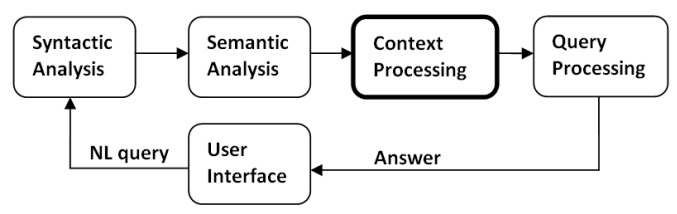
\includegraphics[width=.7\textwidth]{ch03/assets/contextual_nlidb.jpg}
    \caption{Sistema \glsfirst{ilnbd} contextual, extraído de~\textcite{novel_approach_towards_incorporating_context_processing_nlidb}}
    \label{fig:contextual_nlidb}
\end{figure}

Relativamente às abordagens ou estratégias de desenvolvimento deste tipo de \textit{software}, são várias e cada uma delas apresentam particularidades que podem influenciar a forma como o sistema é desenhado~\parencite{nlidb_brief_review, survey_nlidb}:

\begin{itemize}
    \item 
    {
        \textit{Abordagem simbólica (baseada em regras)} -- a linguagem é analisada e é aplicada lógica baseada em regras, de forma a capturar o significado da linguagem. O conhecimento encontra-se mapeado em regras ou noutras formas de representação;
    }
    \item
    {
        \textit{Abordagem empírica (baseada em experiências}) -- aplica análise estatística ou outro tipo de análises orientadas aos dados. Maior parte dos métodos de \gls{pln} aplicam técnicas estatísticas com modelos \textit{n-gram}, \textit{Hidden Markov} ou gramáticas de contexto livre;
    }
    \item
    {
        \textit{Abordagem de conexão (baseado em redes neuronais)} -- baseada em representações distribuídas que correspondem a regularidades estatísticas na linguagem. Uma vez que as capacidades da linguagem humana assentam na rede neuronal no cérebro, as redes neuronais artificiais apresentam um ponto fulcral na modelação do processamento de linguagem.
    }
\end{itemize}

Quanto à arquitetura dos sistemas \gls{ilnbd}, além de serem variadas, possuem também diferentes interpretações ao problema. Cada uma apresenta vantagens e desvantagens, pelo que é necessário explorar, de forma resumida, as características de cada.

\subsubsection{Sistemas \textit{Pattern Matching}}
Os primeiros esforços no desenvolvimento de sistemas deste género começaram em meados do século XX. O conceito de \textit{Pattern Matching} permite mapear diretamente o \textit{input} do utilizador para a obter o resultado desejado. A implementação destes sistemas implica que os detalhes da base de dados estejam presentes no código, ou seja, torna a solução limitada a um contexto específico e ao número e complexidade de padrões existentes~\parencite{nlidb_brief_review}. A principal vantagem desta abordagem prende-se à simplicidade de implementação, pelo que não há necessidade em conceber módulos de interpretação ou \textit{parsing} da linguagem~\parencite{nlidb_brief_review, survey_nlidb}.

\subsubsection{Sistemas Baseados em Sintaxe}
Os sistemas baseados em sintaxe possibilitam que a \inquotes{questão} do utilizador seja analisada sintaticamente, dando origem a uma árvore que é diretamente mapeada para uma expressão \gls{sql}. Para isso, estes sistemas usam uma gramática que descreve as estruturas sintáticas das perguntas dos utilizadores~\parencite{nlidb_brief_review}. Geralmente, é difícil mapear todas regras que constituem a gramática e o processo de escolha de quais as regras devem ser representadas é complexo. Outro problema é o facto de uma frase poder ter múltiplas corretas árvores de análise sintática, que aquando traduzidas, podem levar a diferentes resultados. Também a dificuldade de transformar a árvore de análise sintática diretamente numa linguagem genérica de base de dados é um problema complexo de resolver~\parencite{survey_nlidb}. A principal vantagem desta abordagem é o facto de fornecer informação acerca da estrutura frásica, possibilitando o mapeamento da semântica em regras produtivas (nós da árvore de análise sintática)~\parencite{nlidb_brief_review}.

\subsubsection{Sistemas de Gramática Semântica}
Apesar da sua semelhança com os sistemas baseados em sintaxe, a ideia inerente a um sistema deste tipo é a simplificar a árvore de análise sintática, através da combinação de alguns nós ou remoção dos mesmos. Posto isto, um sistema de gramática semântica é capaz de refletir melhor a representação semântica da frase, sem as estruturas complexas na árvore, com a possibilidade de designar nomes para os nós, reduzindo a ambiguidade. As principais desvantagens desta abordagem prendem-se com a necessidade de conhecimento prévio do domínio, tornando-se difícil a transposição para um outro e a estrutura específica das árvores de análise sintática não poderia ser usado noutra aplicação~\parencite{survey_nlidb, nlidb_brief_review}.

\subsubsection{Sistemas de Representação Intermediária de Linguagem}
Atualmente, os sistemas \gls{ilnbd} transformam a linguagem natural numa representação intermediária, definida internamente. Assim, a \textit{query} lógica representada na linguagem intermédia expressa o significado da questão colocada pelo utilizador em termos dos conceitos do domínio, os quais são independentes da estrutura da base de dados. Posteriormente, a \textit{query} lógica é traduzida na linguagem genérica de base de dados e avaliada. Esta arquitetura surgiu da dificuldade de traduzir diretamente a linguagem natural para a \gls{sql}, ou outra semelhante. O processo de transformação da \textit{query} lógica para a linguagem de base de dados pode conter várias fases, dependendo da necessidade do sistema~\parencite{nlidb_brief_review}.